\documentclass{article} 
\usepackage{geometry}
\usepackage{url}
\geometry{left=3.5cm, right=3.5cm, top=2.5cm, bottom=2.5cm}
\usepackage{graphicx} 
\usepackage[round]{natbib}
\bibliographystyle{plainnat}
\usepackage{amsmath,amsthm}
\usepackage{amsmath}
\usepackage{mhchem}
\usepackage{multirow}

\begin{document}  
\title{621-Final}
\author{Liting Hu}

\maketitle
\tableofcontents

\# Problem A is coded by Matlab. Problem B \& C are by R.
\section{Problem A.}
\subsection{a}
The price of a geometric Asian option in the Black-Scholes model is given by function:

\begin{verbatim}
function [Price] = Black_Scholes_Asian(S0, K, Tm, r, sigma)
% geometric Asian Call option in the Black-Scholes model
% S0: Initial stock price
% K: Strike price
% Tm: Time to maturity
% r: Interest rate
% sigma: Volatility

N = Tm*252;
sigmahat = sigma*sqrt((2*N+1)/6/(N+1));
rho = (r-sigma^2/2+sigmahat^2)/2;
d1 = (log(S0/K) + (rho+sigmahat^2/2)*Tm)/sqrt(Tm)/sigmahat;
d2 = (log(S0/K) + (rho-sigmahat^2/2)*Tm)/sqrt(Tm)/sigmahat;
Price = exp(-r*Tm)*(S0*exp(rho*Tm)*normcdf(d1)-K*normcdf(d2));
\end{verbatim}
The price of geometric Asian call option is 15.1711.

\subsection{b, c}
For b \& c, define function ``Monte\_Carlo\_Asian'' to calculate arithmetic or geometric Asian call options.
\begin{verbatim}
function [Price, lower_bound, upper_bound, Time] = Monte_Carlo_Asian(type, S0, K, Tm, r, sigma, n, m, cl)
% Type=1: arithmetic Asian call options; Type=2: geometric Asian Call
% options
% S0: Initial stock price
% K: Strike price
% Tm: Time to maturity
% r: Interest rate
% sigma: Volatility
% n: Time steps
% m: Quantity of trials
% cl: Confidence level 

tic;
dt = Tm/n;
S0 = ones(1,m).*S0;

if type==1
    sumST = S0;
else
    productST = S0.^(1/(n+1));
end

lnS_T = log(S0);
nudt = (r-sigma^2/2)*dt;
sigsdt = sigma*sqrt(dt);

for i=1:n
    epsilon = normrnd(0,1,1,m);
    dS = nudt+sigsdt.*epsilon; % evolve the stock price
    lnS_T = lnS_T+dS;
    if type==1
        sumST = sumST + exp(lnS_T);
    else
        productST = productST.*exp(lnS_T).^(1/(n+1));
    end
end


if type==1
    profits = max(sumST/(n+1) - K, 0);
else
    profits = max(productST - K, 0);
end

Price = mean(profits)*exp(-r*Tm);
SD = std(profits);
SE = SD/sqrt(m);

z=-norminv((1-0.95)/2);
lower_bound = Price - z*SE;
upper_bound = Price + z*SE;

Time=toc;
\end{verbatim}

For 95\% confidence level:
\begin{table}[h]
\begin{tabular}{|c|c|c|c|c|}

\hline
& Price & Lower & Upper & Time(s) \\
\hline
Arithmetic & 17.4430 & 17.3732 & 17.5129 & 38.0919 \\
\hline
Geometric & 15.1380 & 15.0776 & 15.1983 & 79.3466 \\
\hline

\end{tabular}
\end{table}
The second and third columns indicate the lower and upper bound of confidence intervals.

For 99\% confidence level:

\begin{table}[h]
\begin{tabular}{|c|c|c|c|c|}

\hline
& Price & Lower & Upper & Time(s) \\
\hline
Arithmetic & 17.4873 & 17.4173 & 17.5573 & 37.8842 \\
\hline
Geometric & 15.1747 & 15.1141 & 15.2353 & 76.0741 \\
\hline

\end{tabular}
\end{table}


\begin{verbatim}

\end{verbatim}

\subsection{d}
With same exact random variables:
\begin{verbatim}
function [Price_A, Price_G, b_star] = Monte_Carlo_Asian_duo(S0, K, Tm, r, sigma, n, m)
% Pricing arithmetic and geometric Asian Call with same random variables
% options
% S0: Initial stock price
% K: Strike price
% Tm: Time to maturity
% r: Interest rate
% sigma: Volatility
% delta: Continuous dividend rate
% n: Time steps
% m: Quantity of trials
dt = Tm/n;
S0 = ones(1,m).*S0;

sumST = S0;
productST = S0.^(1/(n+1));

lnS_T = log(S0);
nudt = (r-sigma^2/2)*dt;
sigsdt = sigma*sqrt(dt);

for i=1:n
    epsilon = normrnd(0,1,1,m);
    dS = nudt+sigsdt.*epsilon; % evolve the stock price
    lnS_T = lnS_T+dS;
    sumST = sumST + exp(lnS_T);
    productST = productST.*exp(lnS_T).^(1/(n+1));
end

Yi = max(sumST/(n+1) - K, 0);
Xi = max(productST - K, 0);

Price_A = mean(Yi)*exp(-r*Tm);
Price_G = mean(Xi)*exp(-r*Tm);

Xbar = mean(Xi); Ybar = mean(Yi);
b_star = sum((Xi-Xbar).*(Yi-Ybar))/sum((Xi-Xbar).^2);
\end{verbatim}

And with different M, results are showed below

\begin{table}[h]
\begin{tabular}{|c|c|c|c|}

\hline
M & Price\_Arithmetic & Price\_Geometric & b* \\
\hline
10000 & 17.0118 & 14.7919 & 1.1447  \\
\hline
100000 & 17.4747 & 15.1685 & 1.1514  \\
\hline
500000 & 17.5038 & 15.1831 & 1.1515  \\
\hline
1000000 & 17.5015 & 15.1911 & 1.1503  \\
\hline

\end{tabular}
\end{table}
With M growing higher, ${b^*}$ doesn't vary much and is staying around 1.5.

\subsection{e}
\begin{verbatim}
S0=100; K=100; Tm=5; r=0.03; sigma=0.3;
[Price_G] = Black_Scholes_Asian(S0, K, Tm, r, sigma)
type=2; n=252*5; m=1e6; cl=0.99;
[Price_G_sim, lower_bound, upper_bound, Time] = Monte_Carlo_Asian(type, S0, K, Tm, r, sigma, n, m, cl)
error_G = Price_G - Price_G_sim
\end{verbatim}
The error is 0.0180.

\subsection{f}

\begin{verbatim}
Price_A_star = Price_A_sim - b_star*error_G;
\end{verbatim}

\begin{table}[h]
\begin{tabular}{|c|c|}

\hline
$P_a^{sim}$ & $P_a^*$  \\
\hline
17.4873 &  17.4667  \\
\hline

\end{tabular}
\end{table}

The difference between $P_a^{sim}$ and $P_a^*$ is very small. 

\section{Problem B.}
\subsection{1}
The SPDR ETF I chose is XLF(Financial Select Sector SPDR Fund). 20 equities are 20 top holdings in XLF which are: \\
JPM	JP Morgan Chase \& Co\\
BRK-B	Berkshire Hathaway B\\
WFC	Wells Fargo \& Co\\
BAC	Bank of America Corp\\
C	Citigroup Inc\\
GS	Goldman Sachs Group Inc\\
USB	US Bancorp\\
CB	Chubb Limited\\
MS	Morgan Stanley\\
AXP	American Express Co\\
PNC	PNC Finl Services Group\\
AIG	American Intl Group Inc\\
MET	Metlife Inc\\
BK	The Bank of New York Mellon Corp\\
SCHW	Schwab Charles Corp\\
BLK	BlackRock Inc\\
PRU	Prudential Financial Inc\\
CME	CME Group Inc A\\
COF	Capital One Financial\\
MMC	Marsh \& McLennan Companies\\


Download data:
\begin{verbatim}
sbls <- c("JPM", "BRK-B", "WFC", "BAC", "C", "GS", "USB", "CB", "MS", "AXP", 
          "PNC", "AIG", "MET", "BK", "SCHW", "BLK", "PRU", "CME", "COF", "MMC")
tickers <- data.frame(matrix(ncol = 21, nrow = 1347))
ReturnMatrix <- data.frame(matrix(ncol = 20, nrow = 1347))

for (i in 1:20) {
    sbl <- sbls[i]
    temp <- getSymbols(Symbols = sbl, from = "2012-01-01", to = "2017-05-10", auto.assign = F)
    ReturnMatrix[, i] <- (Cl(temp)-Op(temp))/Op(temp)
    tickers[, (i+1)] <- Cl(temp)
}

tickers[, 1] <- rownames(as.data.frame(temp))
colnames(tickers) <- c("Date", sbls)
colnames(ReturnMatrix) <- sbls
head(tickers)
\end{verbatim}

\begin{figure}[h] 
\begin{center} 
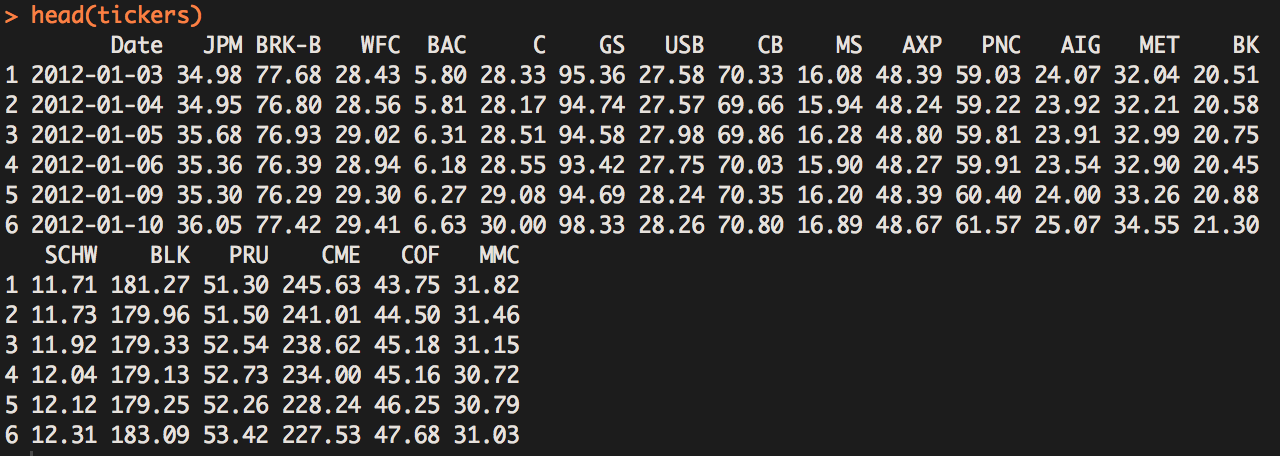
\includegraphics[width = 15cm]{headticker.png}  
\caption{} 
\end{center} 
\end{figure}
 All these prices are above \$5.
 
\begin{verbatim}
# Principal component analysis
tickers.pca <- prcomp(ReturnMatrix, scale. = T)
plot(tickers.pca, type = "l")
pca.summary <- summary(tickers.pca)
pca.summary
# PC7

importance <- as.data.frame(pca.summary$importance)
weight <- importance[2, 1:7]
atic <- abs(tickers.pca$rotation)
stdize <- sweep(atic, 2, colSums(atic), "/")

# Weighted sum of PC1-PC7
weightsum <- atic[, 1:7] %*% matrix(as.numeric(weight), ncol=1)
odr <- order(weightsum, decreasing = T)
order.pca <- stdize[odr, ]
rownames(order.pca)[1:4]
\end{verbatim}

\begin{figure}[h] 
\begin{center} 
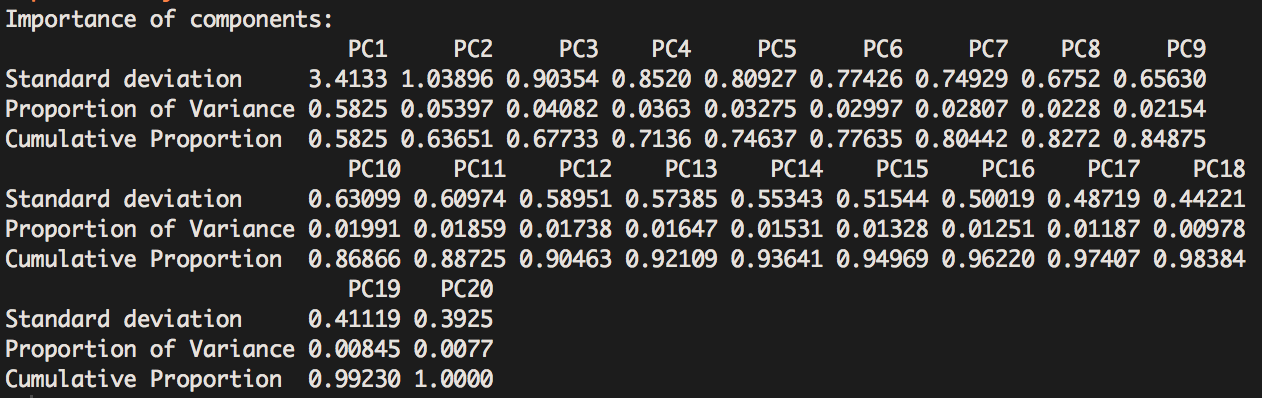
\includegraphics[width = 15cm]{importance.png}  
\caption{Importance of components} 
\end{center} 
\end{figure}
From the summary of PCA, cumulative proportion of variance exceeds 80\% at PC7. So we calculated the weighted sum of absolute value of PC1-PC7 to determine which equities have most contribution to these PCAs. \\

\begin{figure}[h] 
\begin{center} 
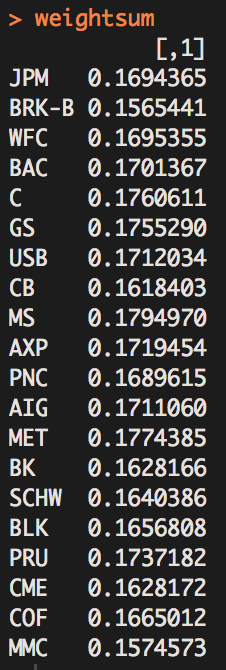
\includegraphics[width = 3cm]{weightsum.png}  
\caption{Weighted sum} 
\end{center} 
\end{figure}

And chose the largest four tickers: ``MS'', ``MET'', ``C'', ``GS''.

\newpage

\subsection{2}
The four stocks I chose are ``JPM'', ``WFC'', ``C'', and ``USB''. \\
Use the AIC criterion and Euler method to choose best model and estimate parameters:
\begin{verbatim}
n <- c(1,3,5,7)
fit.data <- ts(tickers[, (n+1)], deltat=1/255)

model.match <- as.data.frame(matrix(nrow = 4, ncol = 2))
model.match[, 1] <- colnames(fit.data)
best.n <- c()
for (i in 1:4) {
    # model A
    fx1 <- expression( theta[1]*x )
    gx1 <- expression( theta[2]*x )
    mod1 <- fitsde(data=fit.data[, i], drift=fx1, diffusion=gx1,
                   start = list(theta1=.1, theta2=.1), pmle="euler")
    
    # model B
    fx2 <- expression( theta[1]+theta[2]*x )
    gx2 <- expression( theta[3]*x^theta[4] )
    mod2 <- fitsde(data=fit.data[, i], drift=fx2, diffusion=gx2,
                   start = list(theta1=.1,theta2=.1,theta3=.1,theta4=.1), pmle="euler")
    
    # model C
    fx3 <- expression( theta[1]*x )
    gx3 <- expression( theta[2]+theta[3]*x^theta[4] )
    mod3 <- fitsde(data=fit.data[, i], drift=fx3, diffusion=gx3,
                   start = list(theta1=.1,theta2=.1,theta3=.1,theta4=.1), pmle="euler")
    
    # model D
    fx4 <- expression( theta[1]*x )
    gx4 <- expression( theta[2]*x^(3/2) )
    mod4 <- fitsde(data = fit.data[, i], drift=fx4, diffusion=gx4,
                   start = list(theta1=.1,theta2=.1), pmle="euler")
    
    # model E
    fx5 <- expression( theta[1]+theta[2]*x )
    gx5 <- expression( (theta[3]+theta[4]*log(x))*x )
    mod5 <- fitsde(data=fit.data[, i], drift=fx5, diffusion=gx5,
                   start = list(theta1=.1,theta2=.1,theta3=.1,theta4=.1), pmle="euler")
    
    # Computes AIC
    AIC <- c(AIC(mod1),AIC(mod2),AIC(mod3),AIC(mod4),AIC(mod5))
    k <- which.min(AIC)
    best.n[i] <- k
    best <- paste0("model", k)
    model.match[i, 2] <- best
}
model.match # All model 1
\end{verbatim}

\begin{figure}[h] 
\begin{center} 
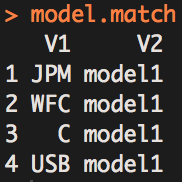
\includegraphics[width = 3cm]{bestmodel.png}  
\caption{Best model match} 
\end{center} 
\end{figure}
All best models are model A (Geometric Black-Scholes).

And then calculated coefficients (${\theta _1},{\theta _2}$) for Monte Carlo:

\begin{verbatim}
# Coefficients
coefs <- data.frame(matrix(nrow = 4, ncol = 3))
coefs[, 1] <- model.match[, 1]

for (i in 1:4) {
    # model A
    fx1 <- expression( theta[1]*x )
    gx1 <- expression( theta[2]*x )
    mod1 <- fitsde(data=fit.data[, i], drift=fx1, diffusion=gx1,
                   start = list(theta1=.1, theta2=.1), pmle="euler")
    coefs[i, 2:3] <- coef(mod1)
}
\end{verbatim}

\begin{figure}[h] 
\begin{center} 
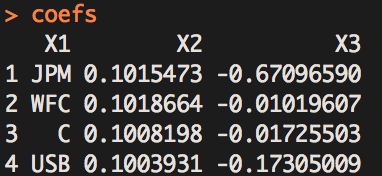
\includegraphics[width = 5cm]{coefs.png}  
\caption{coefficients} 
\end{center} 
\end{figure}

\subsection{3}

The correlation matrix:
\begin{verbatim}
corrmatrix <- cor(fit.data)
corrmatrix
\end{verbatim}

\begin{figure}[h] 
\begin{center} 
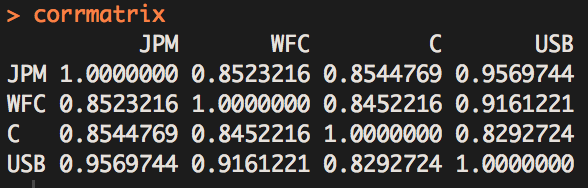
\includegraphics[width = 8cm]{corr.png}  
\caption{correlation matrix} 
\end{center} 
\end{figure}

\subsection{4}
Monte-Carlo:
\begin{verbatim}
S0 <- fit.data[1, ]
monte_carlo_corr <- function(S0, Tm=1, dt=1/255, n=1000, corr=corrmatrix) {
    # S0: Initial stock prices
    # Tm: Time to maturity
    # dt: Time interval
    # n:  Quantity of paths
    # corr: Correlation matrix
    R <- chol(corrmatrix)
    L <- t(R)
    STj <- data.frame(matrix(ncol = 4, nrow = n))
    for (j in 1:n) {
        dZt <- matrix(rnorm(4*Tm/dt)*sqrt(dt), nrow = 4)
        dWt <- L %*% dZt
        
        St <- S0
        
        for (i in 1:(Tm/dt)) {
            drift <- St*coefs[, 2]*dt
            diffusion <- coefs[, 3]*dWt[, i]
            diffusion[1] <- diffusion[1]*St[1]
            diffusion[2] <- diffusion[2]*St[2]
            diffusion[3] <- diffusion[3]*St[3]
            diffusion[4] <- diffusion[4]*St[4]
            St <- St + drift + diffusion
        }
        STj[j, ] <- St
    }
    return(STj)
}
STj <- monte_carlo_corr(S0)
STj

\end{verbatim}
\begin{figure}[h] 
\begin{center} 
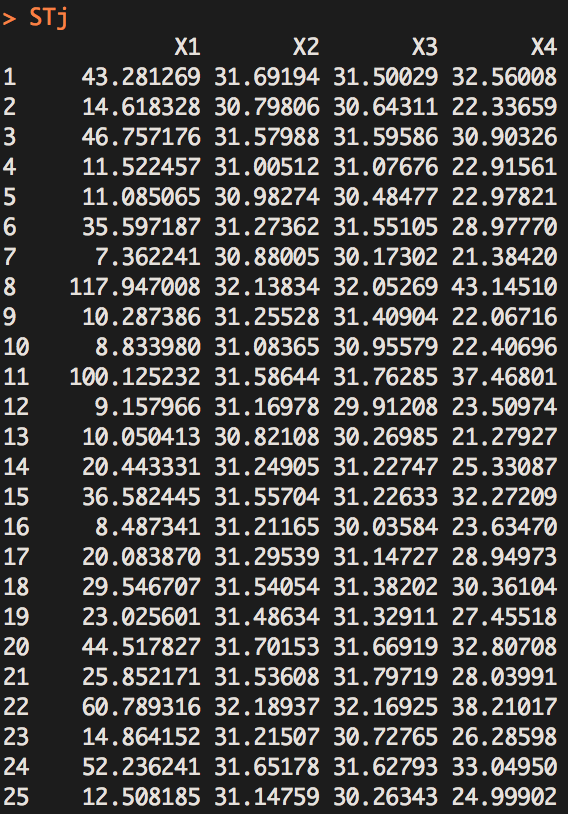
\includegraphics[width = 10cm]{ST.png}  
\caption{n simulations of ST} 
\end{center} 
\end{figure}

\begin{verbatim}
statistics <- do.call(data.frame, 
                      list(mean = apply(STj, 2, mean),
                           sd = apply(STj, 2, sd),
                           skewness = apply(STj, 2, skewness),
                           kurtosis = apply(STj, 2, kurtosis)))
statistics
\end{verbatim}

\begin{figure}[h] 
\begin{center} 
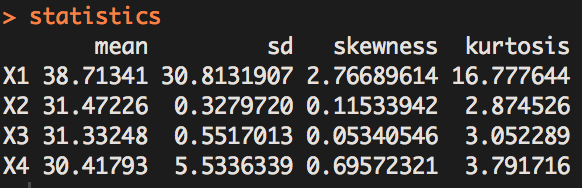
\includegraphics[width = 8cm]{stas.png}  
\caption{Basic statistics} 
\end{center} 
\end{figure}


\subsection{5}
Fit XLF:
\begin{verbatim}
XLF <- getSymbols(Symbols = "XLF", from = "2012-01-01", to = "2017-05-10", auto.assign = F)
XLF.close <- ts(as.numeric(XLF$XLF.Close), deltat=1/255)

# model A - geometric Brownian motion
fx1 <- expression( theta[1]*x )
gx1 <- expression( theta[2]*x )
mod1 <- fitsde(data=XLF.close, drift=fx1, diffusion=gx1,
               start = list(theta1=.1, theta2=.1), pmle="euler")
coef(mod1)
\end{verbatim}

\begin{figure}[h] 
\begin{center} 
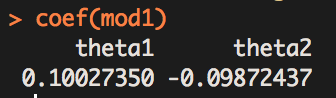
\includegraphics[width = 4cm]{coefx.png}  
\caption{Coefficients from XLF fit} 
\end{center} 
\end{figure}

$\mu$ is 0.10027350 and $\sigma$ is -0.09872437. And then do Monte carlo:

\begin{verbatim}
S0 <- XLF.close[1]
monte_carlo <- function(S0, Tm=1, dt=1/255, n=1000) {
    ST <- data.frame(matrix(ncol = 1, nrow = n))
    for (j in 1:n) {
        dWt <- rnorm(Tm/dt)*sqrt(dt)
        St <- S0
        
        for (i in 1:(Tm/dt)) {
            drift <- St*coef[1]*dt
            diffusion <- St*coef[2]*dWt[i]
            St <- St + drift + diffusion
        }
        ST[j, 1] <- St
    }
    return(ST)
}
XLF.MC <- monte_carlo_corr(S0)
XLF.MC[, 1]

MCsimulations <- cbind(STj, XLF.MC[, 1])
colnames(MCsimulations) <- c("JPM", "WFC", "C", "USB", "XLF")
write.csv(MCsimulations, file = "MCsimulations.csv", row.names = F)
\end{verbatim}
All $S_T$ are saved in a csv file ``MCsimulations.csv''.


\subsection{6}
Linear multivariate regression:
\begin{verbatim}
Multivariate.data <- as.data.frame(cbind(fit.data, XLF.close))

lm.fit <- lm(XLF.close~. + 0, data = Multivariate.data)
w <- lm.fit$coefficients
w
\end{verbatim}

\begin{figure}[h] 
\begin{center} 
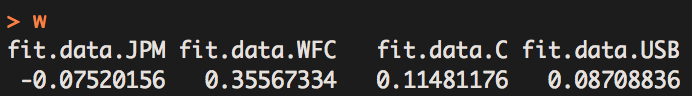
\includegraphics[width = 10cm]{reg.png}  
\caption{Linear multivariate regression} 
\end{center} 
\end{figure}

\subsection{7}
\begin{verbatim}
basket <- MCsimulations # Weighted ST
for (i in 1:4) {
    basket[, i] <- MCsimulations[, i]*w[i]
}

mean(pmax(rowSums(basket) - MCsimulations[, 5], 0))
mean(pmax(MCsimulations[, 5] - rowSums(basket), 0))
\end{verbatim}

\begin{figure}[h] 
\begin{center} 
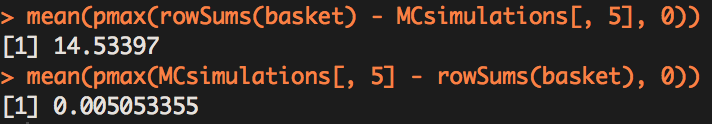
\includegraphics[width = 10cm]{P27.png}  
\caption{Linear multivariate regression} 
\end{center} 
\end{figure}

The premium of ${(\sum\limits_{i = 1}^4 {{w_i}{S_i}(T) - {S_T}} )_ + }$ is 14.53397. While the premium of ${({S_T} - \sum\limits_{i = 1}^4 {{w_i}{S_i}(T)} )_ + }$ is 0.005053355.

\section{Problem C.}
Firstly, we need to process data:
\begin{verbatim}
# Dealing with data -------------------------------------------------------

library(xlsx)
SPX <- read.xlsx("SPX.xls", sheetName = "QuoteData-1", header=F) # read data
SPX <- SPX[colSums(!is.na(SPX)) > 0] # omit NA columns
SPX <- SPX[rowSums(!is.na(SPX)) > 0, ] # omit NA rows
date0 <- as.numeric(as.character(SPX[1, 1])) 
price0 <-as.numeric(as.character(SPX[1, 2])) 
r0 <- as.numeric(as.character(SPX[1, 3]))/100 
div <- 0

colnames(SPX) <- c("Date", "Tm", "K", "Price")
SPX <- SPX[-c(1, 2), ]
for (i in 1:4) { # Convert factor to numeric
    SPX[, i] <- as.numeric(as.character(SPX[, i]))
}
SPX <- SPX[!duplicated(SPX[, 2:3], fromLast = T), ]

head(SPX)
\end{verbatim}

It's like

\begin{figure}[h] 
\begin{center} 
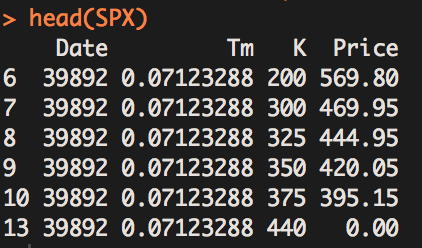
\includegraphics[width = 6cm]{SPX.png}  
\caption{Head of SPX} 
\end{center} 
\end{figure}

\subsection{a}

Pricing by BS formula:
\begin{verbatim}
Option_BSM <- function(S0, K, Tm, sigma, r=r0, div=0) {
    # Pricing by Black Scholes
    d1 <- (log(S0/K) + (r - div + sigma^2/2)*Tm)/sigma/sqrt(Tm)
    d2 <- d1 - sigma*sqrt(Tm)
    p <- S0*exp(-div*Tm)*pnorm(d1) - K*exp(-r*Tm)*pnorm(d2)
    return(p)
}
\end{verbatim}

Functions to calculate implied volatilities
\begin{verbatim}
fsigma <- function(sigma, Tm, K, price) {
    # Epsilon. To calculate implied vol
    S0 <- price0
    price.by.bs <- Option_BSM(S0, K, Tm, sigma)
    ans <- price.by.bs - price
    return(ans)
}

imp_vol <- function(Tm, K, price) {
    # use bisection method to calculate implied volatility
    a <- 0.0001
    b <- 10
    epsilon <- abs(a - b)
    while(epsilon > 1e-4) {
        mid <- (a + b)/2
        if (fsigma(mid, Tm, K, price)*fsigma(b, Tm, K, price) < 0 ) a <- mid
        else b <- mid
        epsilon <- abs(a - b)
    }
    return(a)
}
Implied_Vol <- SPX[, 1]
for(i in 1:nrow(SPX)) {
    price <- SPX[i, 4]
    Tm <- SPX[i, 2]
    K <- SPX[i, 3]
    Implied_Vol[i] <- imp_vol(Tm, K, price)
}
newdf <- data.frame(SPX[, -1], Implied_Vol)
newdf <- subset(newdf, Implied_Vol>0.0001) #eliminate meaningless implied vol
head(newdf)
\end{verbatim}

To find 20 different strike prices and 4 different maturities:
\begin{verbatim}
todr <- order(table(newdf$Tm), decreasing = T)[1:4]
T1 <- as.numeric(names(table(newdf$Tm)[todr]))

K1 <- newdf$K[newdf$Tm==T1[1]]
K2 <- newdf$K[newdf$Tm==T1[2]]
K3 <- newdf$K[newdf$Tm==T1[3]]
K4 <- newdf$K[newdf$Tm==T1[4]]
common_element=intersect(intersect(K1,K2),intersect(K3,K4))[1:20]

dfselect <- subset(newdf, Tm %in% T1 & K %in% common_element)
a <- order(dfselect[, 1], dfselect[, 2])
dfselect <- dfselect[a, ]

if (nrow(dfselect) < 80) {print("No enough option data")}
\end{verbatim}

Data frame dfselect contains 20*4 entries. \\

The 3D plot for $\{ {K_i},{T_j},{\sigma _{ij}}\} $ is showed below:

\begin{figure}[h] 
\begin{center} 
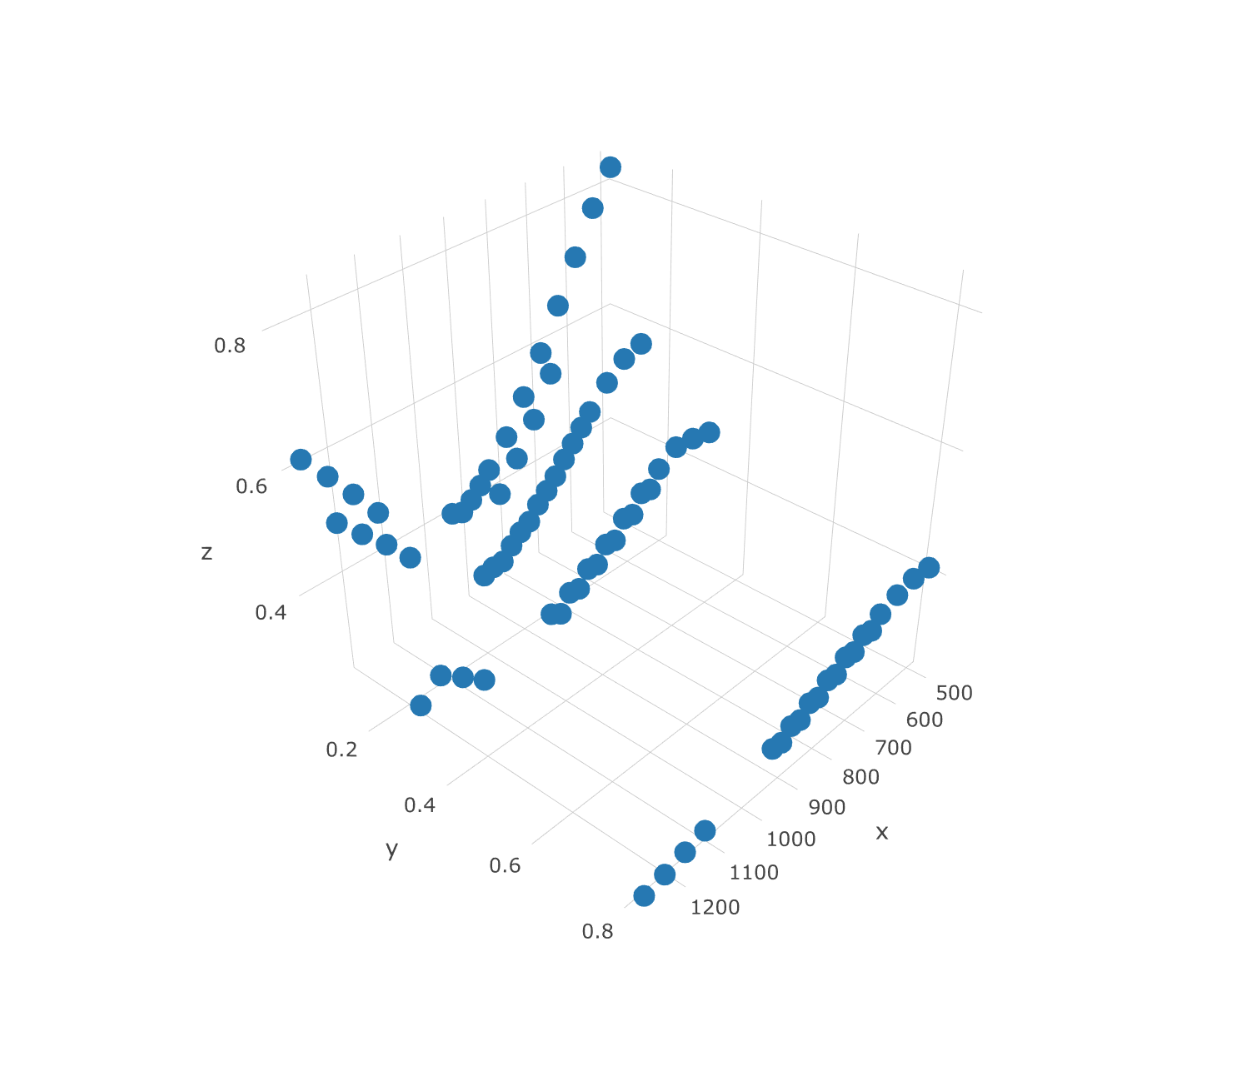
\includegraphics[width = 10cm]{imp2.png}  
\caption{Implied vols} 
\end{center} 
\end{figure}

\subsection{b}

Using linear interpolation:
\begin{verbatim}
library(akima)
library(rgl)
x <- dfselect$K #+ seq(0, 0.0001, length.out = n)
y <- dfselect$Tm #+ seq(0, 0.0001, length.out = n)
z <- dfselect$Implied_Vol

# linear interpolation
n_interpolation <- 200
spline_interpolated <- interp(x, y, z,
                              xo=seq(min(x), max(x), length = n_interpolation),
                              yo=seq(min(y), max(y), length = n_interpolation),
                              linear = T)

x.si <- spline_interpolated$x
y.si <- spline_interpolated$y
z.si <- spline_interpolated$z
plot_ly(x=x.si, y=y.si, z=z.si, type = "surface")
\end{verbatim}

\begin{figure}[h] 
\begin{center} 
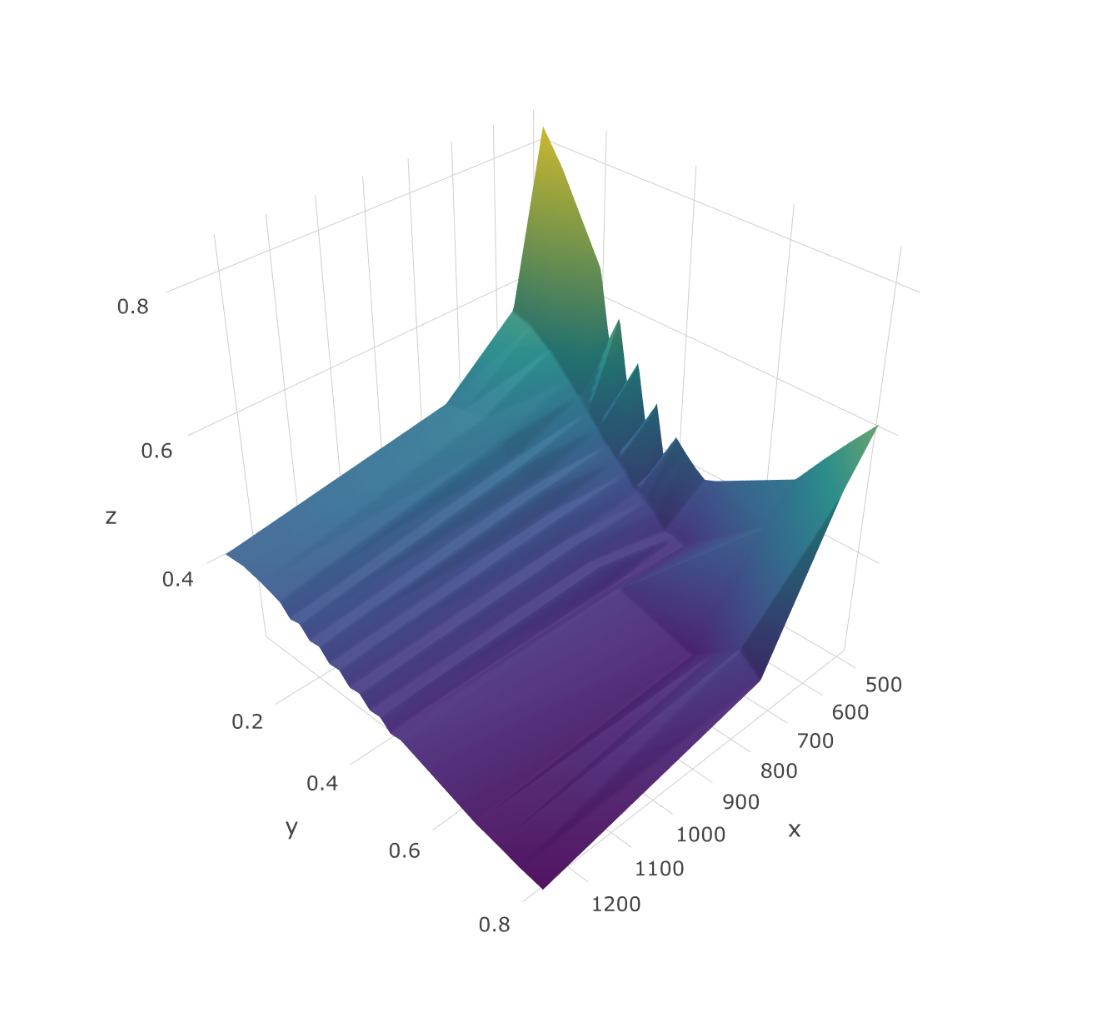
\includegraphics[width = 13cm]{int.png}  
\caption{Interpolation surface} 
\end{center} 
\end{figure}

\subsection{c}
I don't think that non-arbitrage condition holds in the surface. Cause what I do is interpolating linearly, for calculated points on the surface, their volatilities are estimated higher, which means the call option prices considered higher then expected. So arbitrage exists that one can buy call option in these point and sell to the market.


\subsection{d}
Calculate square of local volatility:
\begin{verbatim}
# local volatility

local_vol <- function(Tm, K, price) {
    # Square of local volatility
    S0 <- price0
    deltaT <- 0.001*Tm
    deltaK <- 0.001*K
    sig <- imp_vol(Tm, K, price)
    d1 <- (log(S0/K) + (r0 - div + sig^2/2)*(Tm))/sig/sqrt(Tm)
    dT1 <- (imp_vol(Tm+deltaT, K, price) - imp_vol(Tm, K, price))/deltaT
    dK1 <- (imp_vol(Tm, K+deltaK, price) - imp_vol(Tm, K, price))/deltaK
    dK2 <- (imp_vol(Tm, K+deltaK, price) - 2*imp_vol(Tm, K, price)
            + imp_vol(Tm, K-deltaK, price))/deltaK^2
    numerator <- 2*sig*dT1*Tm + sig^2 + 2*sig*(r0-div)*Tm*K*dK1
    denominator <- (1 +K*d1*dK1*sqrt(Tm))^2 + K^2*Tm*sig*(dK2 - d1*dK2^2*sqrt(Tm))
    lsigma <- numerator/denominator
    return(lsigma)
}

Local_Vol <- dfselect[, 1]
for(i in 1:nrow(dfselect)) {
    # calculate local vols
    price <- dfselect[i, 3]
    Tm <- dfselect[i, 1]
    K <- dfselect[i, 2]
    Local_Vol[i] <- local_vol(Tm, K, price)
}
head(Local_Vol)
dfselect <- cbind(dfselect, Local_Vol)
\end{verbatim}

\subsection{e}
To price the call option, we need to solve the PDE: $\frac{{\partial C}}{{\partial t}} =  - \frac{{{b^2}(S,t)}}{2}\frac{{{\partial ^2}C}}{{\partial {S^2}}}$

\begin{verbatim}
# Solve the PDE

Tm <- dfselect[1, 1]
K <- dfselect[1, 2]
b <- dfselect[1, 5]
# European Call option - Explicit Finite Difference method
Option_Ex <- function(Tm, K, b, N, Nj) {
    # precompute constants
    dt <- Tm/N
    dx <- 0.2
    
    # initialise asset prices at maturity
    St <- seq(1,2*Nj+1)
    St <- price0 + dx*(St-1-Nj)
    
    # initialise option values at maturity
    C <- matrix(0, ncol = (N + 1), nrow = (2*Nj + 1))
    C[, N+1] <- pmax(C[, N+1], St - K)
    
    # step back 
    for (i in N:1) {
        for(j in (2-i+N):(2*Nj+i-N)) {
            dCdS <- (C[j+1, i+1] - 2*C[j, i+1] + C[j-1, i+1])/dx^2
            dCdt <- -b/2*dCdS
            C[j, i] <- C[j, i+1] - dCdt*dt
        }
    }
    ans <- C[Nj+1, 1]
    return(ans)
}

PricebyD <- dfselect[, 1]
N <- 10000
Nj <- 5000
for(i in 1:nrow(dfselect)) {
    # calculate option price by Dupire?s local vol
    i=1
    Tm <- dfselect[i, 1]
    K <- dfselect[i, 2]
    b <- dfselect[i, 5]
    PricebyD[i] <- Option_Ex(Tm, K, b, N, Nj)
}
\end{verbatim}

\newpage

\subsection{f}
\begin{verbatim}
dfselect <- cbind(dfselect, PricebyD)
write.xlsx(dfselect, "SPXvolatility.xls", row.names = F) # write xlsx file
\end{verbatim}

\begin{figure}[h] 
\begin{center} 
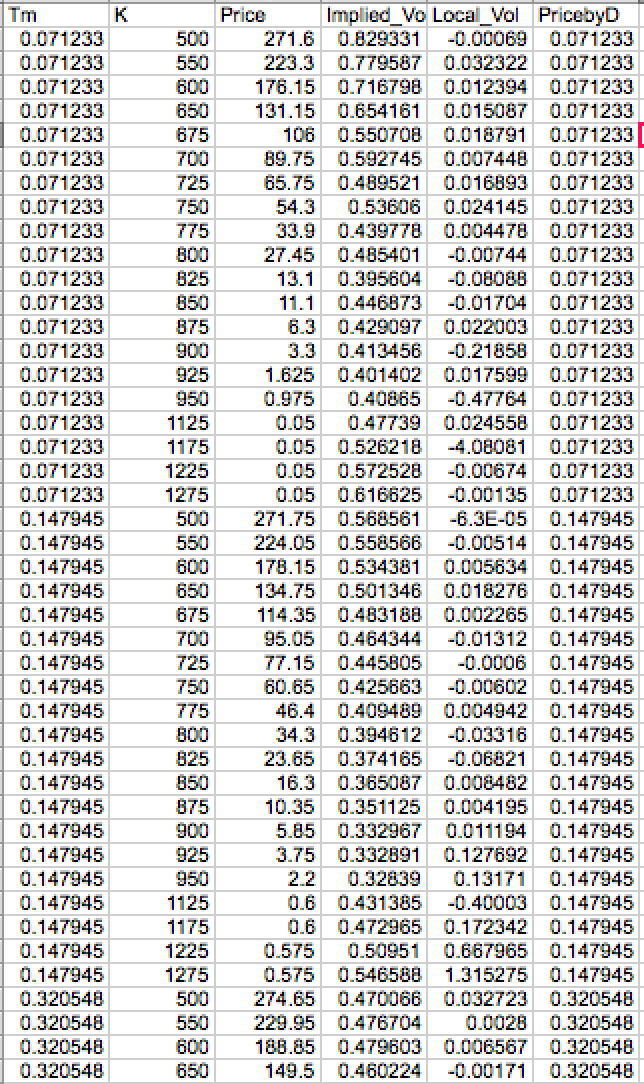
\includegraphics[width = 10cm]{S1.png}  
\caption{SPX results 1} 
\end{center} 
\end{figure}

\begin{figure}[h] 
\begin{center} 
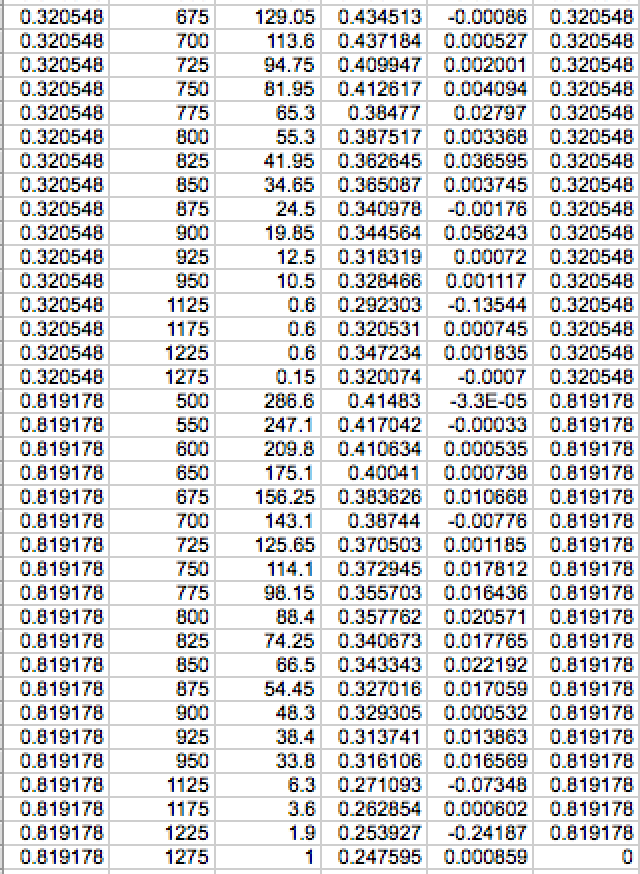
\includegraphics[width = 10cm]{S2.png}  
\caption{SPX results 2} 
\end{center} 
\end{figure}

Sorry for the results of square local vols and Dupire's prices. Although checking my code and formulas from paper several times, I still cannot get reasonable answers. 

\subsection{g}
\begin{verbatim}
# Prepare Data
# Get option chains from Yahoo finance
AAPL.OPTS <- getOptionChain("AAPL", NULL)

D0 <- as.numeric(as.Date("2017/05/15", format="%Y/%m/%d"))

C1 <- AAPL.OPTS$May.19.2017$calls
D1 <- as.numeric(as.Date("2017/05/19", format="%Y/%m/%d"))
T1 <- D1-D0
C1$Date <- D1
C1$Tm <- T1/365

C2 <- AAPL.OPTS$May.26.2017$calls
D2 <- as.numeric(as.Date("2017/05/26", format="%Y/%m/%d"))
T2 <- D2-D0
C2$Date <- D2
C2$Tm <- T2/365

C3 <- AAPL.OPTS$Jun.02.2017$calls
D3 <- as.numeric(as.Date("2017/06/02", format="%Y/%m/%d"))
T3 <- D3-D0
C3$Date <- D3
C3$Tm <- T3/365

C4 <- AAPL.OPTS$Jun.09.2017$calls
D4 <- as.numeric(as.Date("2017/06/09", format="%Y/%m/%d"))
T4 <- D4-D0
C4$Date <- D4
C4$Tm <- T4/365

C5 <- AAPL.OPTS$Jun.16.2017$calls
D5 <- as.numeric(as.Date("2017/06/16", format="%Y/%m/%d"))
T5 <- D5-D0
C5$Date <- D5
C5$Tm <- T5/365

temp <- rbind(C1, C2, C3, C4, C5)
temp$price <- (temp$Bid + temp$Ask)/2

AAPL <- temp[, c(8, 9, 1, 10)]

# Get the actual stock price
todaystock <- getQuote("AAPL") 
S_0 <- todaystock[, 2]

r <- 0.0075
# Treasury bill rate

row0 <- c(D0, S_0, r, NaN)
AAPL <- rbind(row0, c("Date", "T", "K", "Price"), AAPL)
write.xlsx(AAPL, "AAPL.xls", row.names = F, col.names = F) # write xlsx file
\end{verbatim}

\begin{figure}[h] 
\begin{center} 
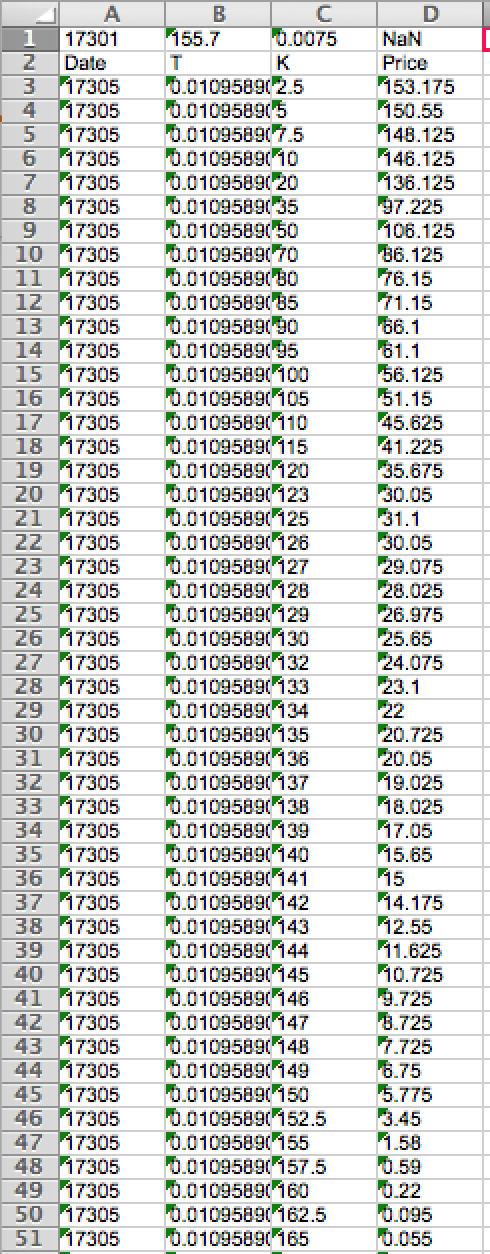
\includegraphics[width = 8cm]{AAPL.png}  
\caption{AAPL options} 
\end{center} 
\end{figure}

\begin{figure}[h] 
\begin{center} 
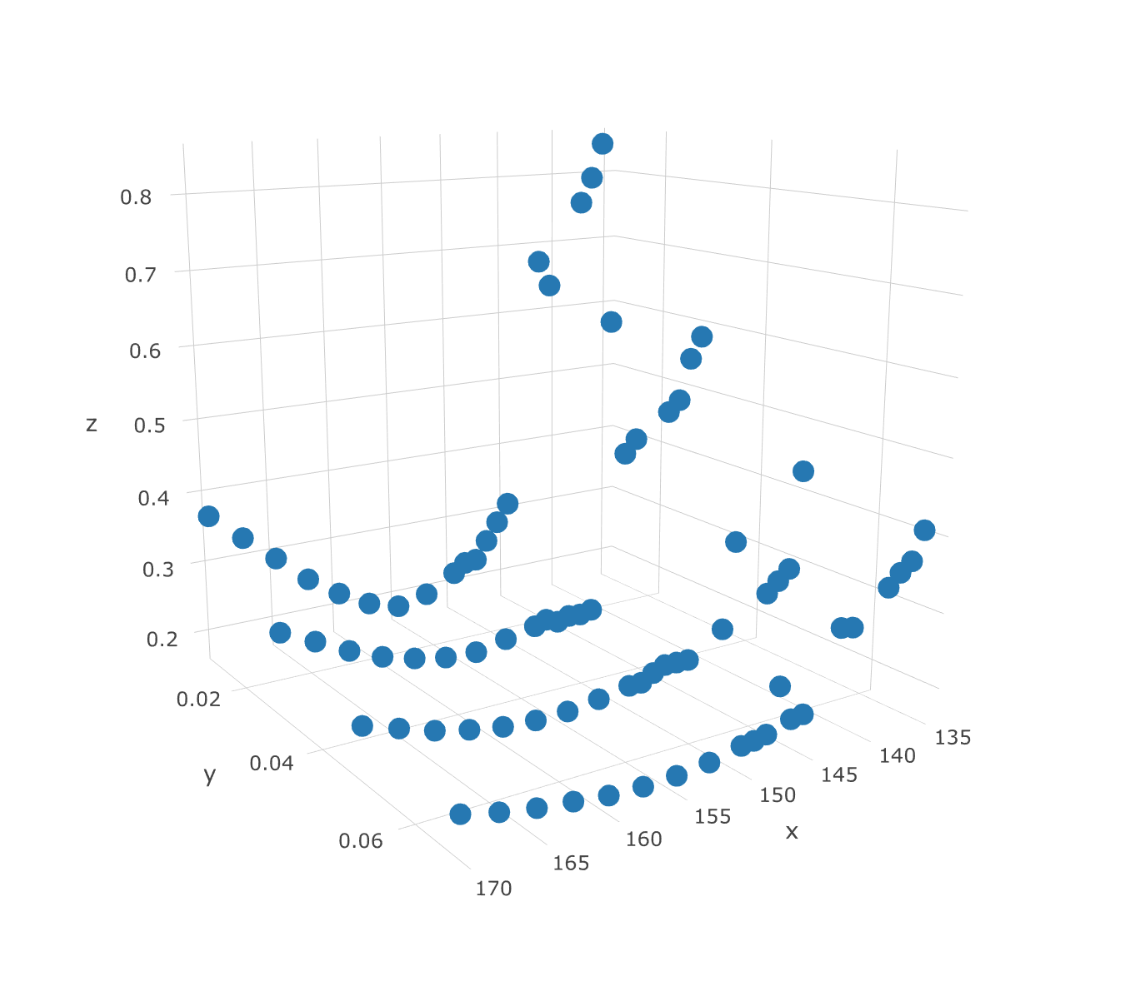
\includegraphics[width = 12cm]{smile.png}  
\caption{AAPL implied volatilities} 
\end{center} 
\end{figure}

\begin{figure}[h] 
\begin{center} 
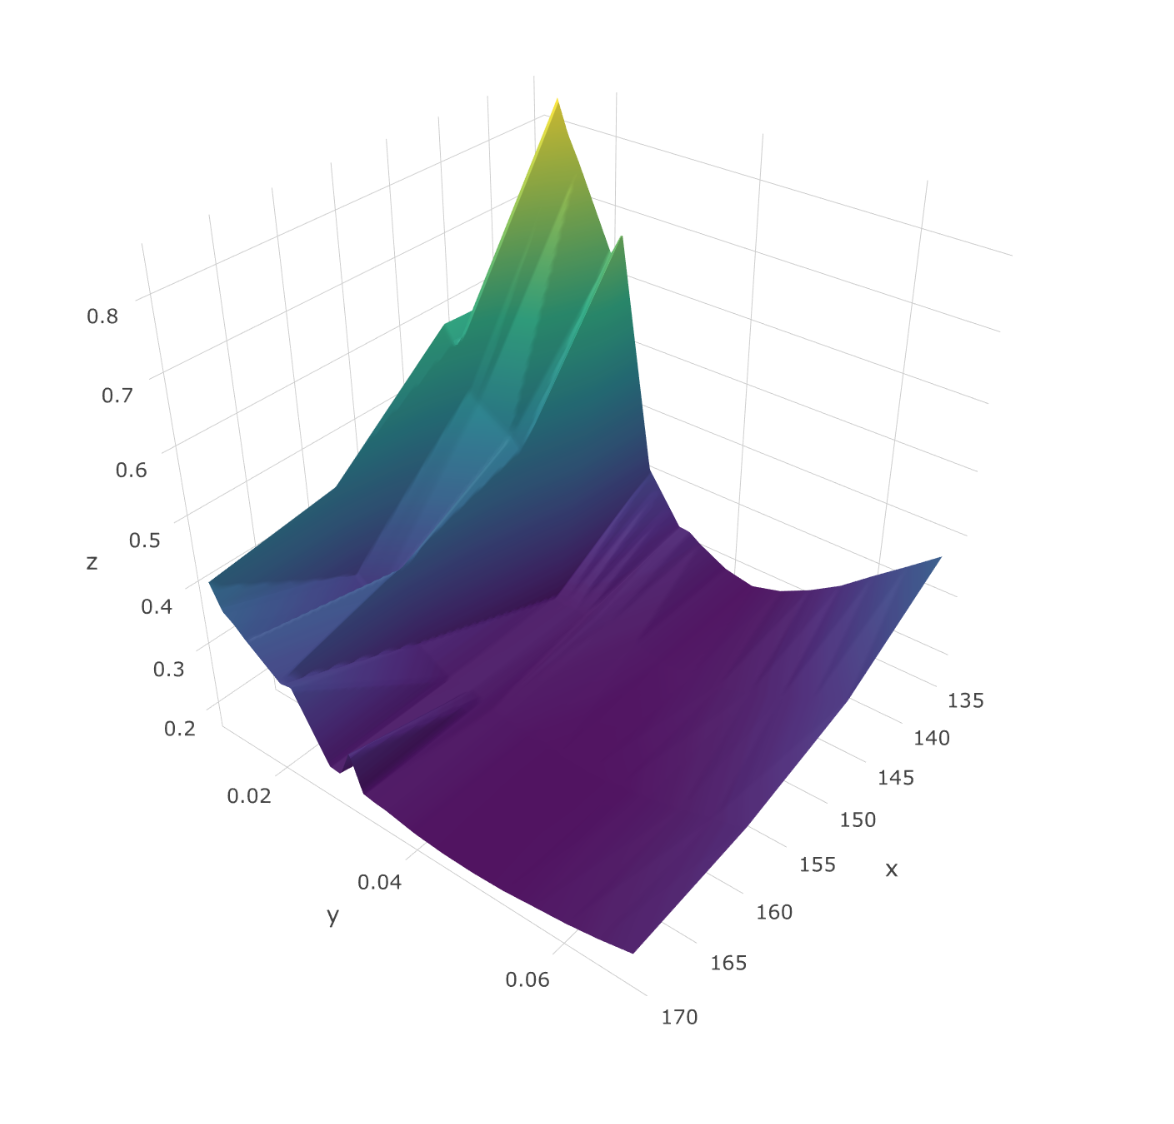
\includegraphics[width = 12cm]{int2.png}  
\caption{AAPL interpolation surface} 
\end{center} 
\end{figure}

\begin{figure}[h] 
\begin{center} 
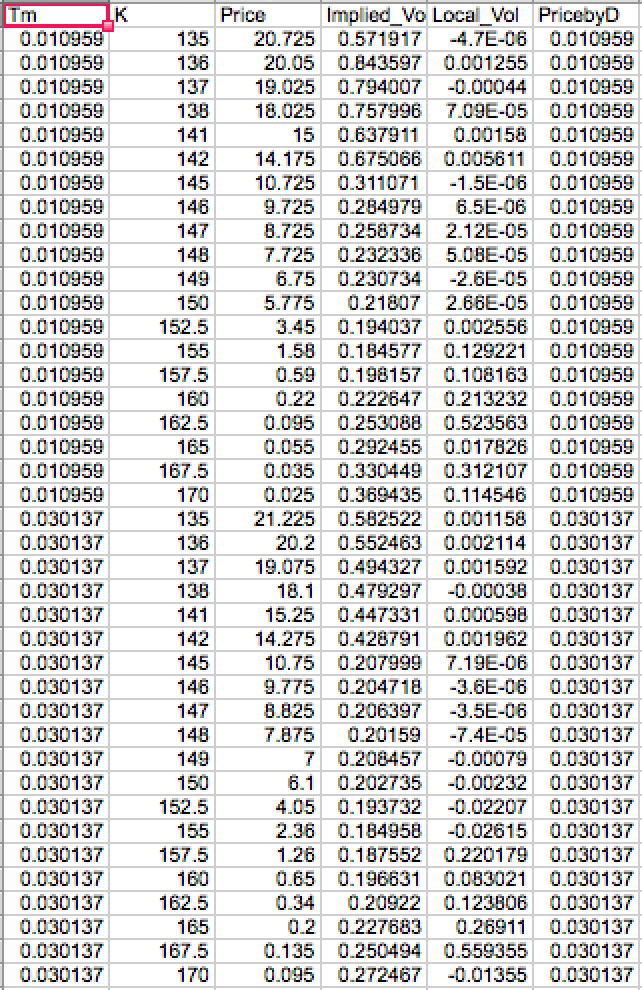
\includegraphics[width = 11cm]{A1.png}  
\caption{AAPL interpolation surface} 
\end{center} 
\end{figure}

\begin{figure}[h] 
\begin{center} 
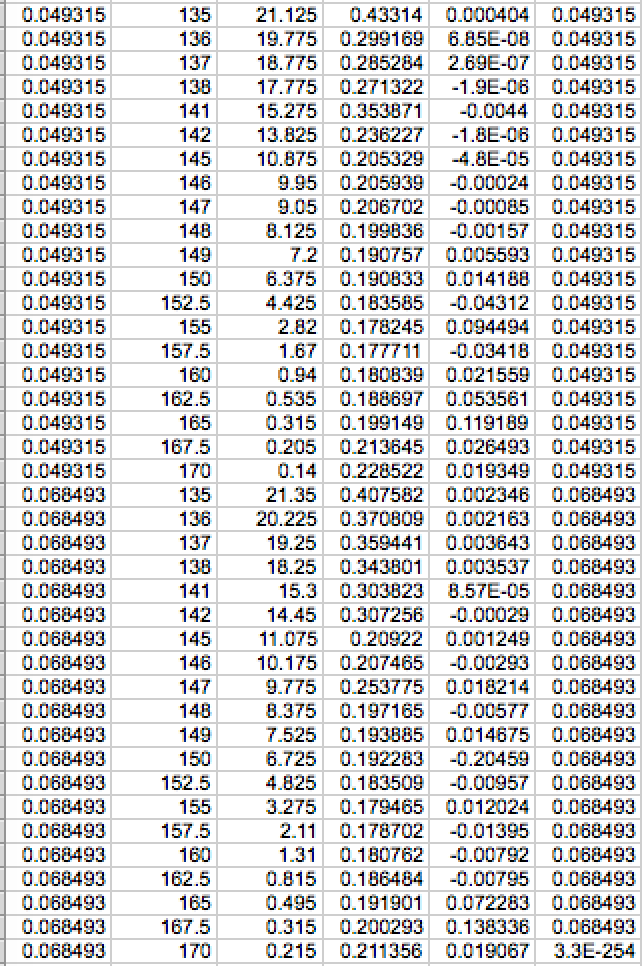
\includegraphics[width = 11cm]{A2.png}  
\caption{AAPL interpolation surface} 
\end{center} 
\end{figure}
\end{document}